\documentclass{deliverablereport}

\usepackage{pdfpages}
\usepackage{multirow}
\usepackage{doi}
\usepackage{hyperref}
\hypersetup{
  colorlinks=true,
  urlcolor=cyan,
  linkcolor=blue,
  citecolor=blue,
}

\deliverable{component-architecture}{hpc-configure}
\deliverydate{XX/YY/201Z}
\duedate{31/08/2019 (M48)}
\author{Alexis Breust, Karim Belabas, Jean-Guillaume Dumas, Jeroen Demeyer, William B. Hart, Steve Linton, Clément Pernet, Hongguang Zhu}

\newcommand{\fflasffpack}{\textsc{fflas-ffpack}\xspace}
\begin{document}
\maketitle
% This will be the abstract, fetched from the github description
\githubissuedescription

% write the report here

\tableofcontents

%%%%%%%%%%%%%%%%%%%%%%%%%%%%%%%%%%%%%%%%%%%%%%%%%%%%%%%%%%%%%%
\section{Introduction}

End-user computational mathematics systems such as \SageMath must deal with 
conflicting constraints such as:
\begin{compactenum}
\item covering a broad, if not exhaustive, range of features,
\item in a high level and user-friendly API,
\item relying on highly tuned dedicated libraries or sub-systems to
  achieve competitive performance.
\end{compactenum}

A common use case of such software is to perform  experimental mathematics,
for e.g. testing conjectures on as many as possible instances with dimensions as
large as possible. In this perspective, users seek for computational efficiency
and the ability to harness the power of high-end HPC servers or clusters.

Work-package 5 has resulted in either enabling or drastically enhancing the high
performance capabilities of several computational mathematics systems
(\longtaskref{hpc}{hpc-pari}, \longtaskref{hpc}{hpc-gap} and
\longtaskref{hpc}{hpc-singular}) or of dedicated libraries
(\longtaskref{hpc}{hpc-linbox}).
%
Based on these results, we now investigate how to expose the HPC capabilities of
those components to the end-user level in the \SageMath system.


%%%%%%%%%%%%%%%%%%%%%%%%%%%%%%%%%%%%%%%%%%%%%%%%%%%%%%%%%%%%%%
\section{Difficulties in composing parallel software systems}

In our  investigations, it appeared that composing a parallel system into
another system was more challenging than anticipated, for several reasons
depending on each system.
\subsection{Using a multi-threaded Singular}

The \Singular system outsources some of its multivariate polynomial arithmetic
to the \texttt{FLINT} library. While a significant effort has been put in the
parallelization of the \texttt{FLINT} library, only part of this code has been
exposed in Singular so far, in particular since \texttt{FLINT} had to adopt
a different API than that of \Singular for representing multivariate
polynomials.

As a consequence, exposing the new parallel multivariate polynomial code in
\SageMath will require us to wait for \Singular to fully leverage \texttt{FLINT},
be released, and then integrated into \SageMath, or the \SageMath
implementation will have to be completely rewritten to directly rely on \texttt{FLINT},
bypassing \Singular.
The latter would require a significant development effort which was not possible
for this deliverable. The former is dependent on a future official release of
Singular.

\subsection{HPC GAP}

A similar situation applies with the progresses on HPC-GAP: for the time being,
the HPC capabilities of GAP are only available through the HPC-GAP platform and
exposing them through the \texttt{libgap} library would require a long effort.

\subsection{Using a multi-threaded \Pari}

As reported in \delivref{hpc}{pari-hpc2}, the number theory library \Pari supports
multi-threading for various operations.
\Sage uses \Pari for its number theory functionality.
Since \Sage simply interfaces \Pari, it should in theory
be trivial to use \Pari-MT (the multi-threading-enabled configuration of \Pari) in \Sage:
just enable multi-threading and that's it.

Unfortunately, some problems arise:
it turns out that \Pari-MT is not compatible with
threads that are created outside of \Pari's control.
So, an application that is already multi-threaded cannot use \Pari-MT without additional effort.
This is in particular a problem for the documentation builder of \Sage,
which uses \Pari to create images for the documentation.
Since this can take a long time, \Sage uses Python's
multiprocessing module for this,
which (perhaps confusingly) also uses multiple threads.

We expect that this problem can be solved with some additional effort
in either the \Sage--\Pari interface or within \Pari itself.
Unfortunately, there was not enough time to further investigate this.

Nevertheless, it is easily possible to use \Pari-MT in \Sage
if one is careful not to build the documentation,
nor to use any other kind of multi-threading.

%%%%%%%%%%%%%%%%%%%%%%%%%%%%%%%%%%%%%%%%%%%%%%%%%%%%%%%%%%%%%%
\section{Exposing the parallel finite field linear algebra library \Linbox}

We were then more successful in exposing the parallel features of the \Linbox
library, and more specifically of its kernel for finite field linear algebra,
\texttt{fflas-ffpack}. By nature, a library is designed with composability in
mind, and thread safety is among the required features a parallel library should
provide.

\subsection{Context}

Finite field linear algebra is a core building block in computational mathematics.
It has a wide range of applications, including number theory, group theory, combinatorics, etc. \SageMath relies on the
\fflasffpack library for its critical linear algebra operations on prime fields of less than 23 bits and consequently
also for numerous computations with multi-precision integer matrices.  

The \fflasffpack library had some preliminary support for multi-core parallelism for matrix
multiplication and Gaussian elimination.
Instead of being tied to a specific parallel language, the library uses a Domain Specific Language, Paladin~\cite{paladin},
to provide the library programmer with unique API for writing parallel code, which is then translated into 
OpenMP~\cite{openmp}, Cilk~\cite{cilk}, Intel-TBB~\cite{tbb}, or XKaapi~\cite{xkaapi} directives. Beside portability and independence from
a given technology, this also makes it possible to benchmark and compare how parallel runtimes perform. This is
particularly important here, since many of the compute intensive routines of \fflasffpack share specificities that are
often challenges for parallel runtime:
\begin{description}
\item[Recursion] by design, sub-cubic linear algebra algorithms are recursive and so are most routines in the
  library.
\item[Heterogeneity] many exact computations must deal with data with size unknown before their actual computation. For
  instance rank deficiencies in Gaussian elimination may generates a block decomposition of varying dimensions and
  therefore computing tasks will have heterogeneous load.
\item[Fine grained task parallelism] the combination of the two above constraints leads to consider recursive task
  fine-grained parallelism, such that a work-stealing engine could efficiently balance the heterogeneity. However,
  recursive tasks have been for a long time rather inefficient in e.g. OpenMP implementations, and the ability to handle
  numerous small tasks is also demanding on parallel runtimes.
\end{description}

\subsection{Integration within \SageMath}

The main tasks for the exposition of the parallel routines of \fflasffpack in \SageMath were the following:
\begin{enumerate}
\item improving existing parallel code for Gaussian elimination and matrix multiplication in the \fflasffpack library;
\item adding new parallel routines in \fflasffpack for the most commonly used operations in \SageMath: the determinant,
  the echelon form, the rank, and the solution of a linear system;
\item connecting these parallel routines in \SageMath  providing  the user
  with a precise control on the number of threads allocated to the linear algebra routines. 
\end{enumerate}

The first two items involved 15 pull-requests, merged and released in
\texttt{fflas-ffpack-2.4.3}\footnote{\url{https://github.com/linbox-team/fflas-ffpack/releases/tag/2.4.3}}. This release
was produced simultaneously with that of the two other libraries in the \Linbox
ecosystem: \texttt{givaro-4.1.1}\footnote{\url{https://github.com/linbox-team/givaro/releases/tag/4.1.1}} and
\texttt{linbox-1.6.3}\footnote{\url{https://github.com/linbox-team/linbox/releases/tag/v1.6.3}} then integrated into \SageMath
in tickets
\begin{itemize}
\item  \url{https://trac.sagemath.org/ticket/26932} and
\item  \url{https://trac.sagemath.org/ticket/27444},
\end{itemize}
which will appear in release 8.9 of \SageMath.

As a side note, the integration of these new releases including the contributions to \delivref{hpc}{LinBox-algo} lead
to a significant speed-up in the sequential computation time of finite field linear algebra in \SageMath, as show in
Table~\ref{tab:release}.
%
\begin{table}[htb]
  \begin{tabular}{lcccc}
    \toprule
&    \multicolumn{2}{c}{$\mathbb{Z}/4\,194\,301\mathbb{Z}$}&    \multicolumn{2}{c}{$\mathbb{Z}/251\mathbb{Z}$}\\
    & Before & After & Before & After\\
    \midrule
    Matrix product & 3.61& 3.57&1.59&1.5 \\
    Determinant &  2.96& 1.52 &1.54&0.731\\
    Echelon form & 3.59& 1.86 & 1.82& 0.692 \\
    Linear system & 8.9 & 5.13 & 3.7&1.79\\ 
    \bottomrule
  \end{tabular}
  \vspace{1em}
  
  \caption{Improvement of the sequential code with \texttt{fflas-ffpack-2.4.3}. Computation time in seconds for a
    $4000\times    4000$ machine over a 22 bits and a 8 bits finite field, on an Intel i7-8950 CPU.}
  \label{tab:release}
\end{table}

For Item (3), we explored several options and chose rely on and extend the Singleton class \texttt{Parallelism} in
\SageMath. This class work as a dictionary registering the number of threads with which each component in \SageMath can
run in parallel.

For example, the following code requires than any linear algebra routine relying on linbox be parallelized on 16 cores.

\begin{lstlisting}
sage: Parallelism().set("linbox",16)
\end{lstlisting}

The following session demonstrates the gain in parallelizing the product of a random $8000\times 8000$ matrix over
$\mathbb{Z}/65521\mathbb{Z}$ with itself using 16 cores:
\begin{lstlisting}
pernet@dahu34:~/soft/sage$ ./sage 
SageMath version 8.9.beta8, Release Date: 2019-08-25
sage: a=random_matrix(GF(65521),8000)
sage: Parallelism()
Number of processes for parallelization:
 - linbox computations: 1
 - tensor computations: 1
sage: time b=a*a
CPU times: user 17.5 s, sys: 1.04 s, total: 18.5 s
Wall time: 18.5 s
sage: Parallelism().set("linbox",16)
sage: Parallelism()
Number of processes for parallelization:
 - linbox computations: 16
 - tensor computations: 1
sage: time b=a*a
CPU times: user 28.9 s, sys: 4.85 s, total: 33.8 s
Wall time: 2.41 s
\end{lstlisting}

Figure~\ref{fig:histo_sage} shows computation time of three high level sage routines
  \texttt{b=a*a},  \texttt{a.determinant()} and \texttt{a.echelon\_form()} on a large square matrix of
order $20000$, with varying number of cores.
\begin{figure}[htb]
  \begin{center}
    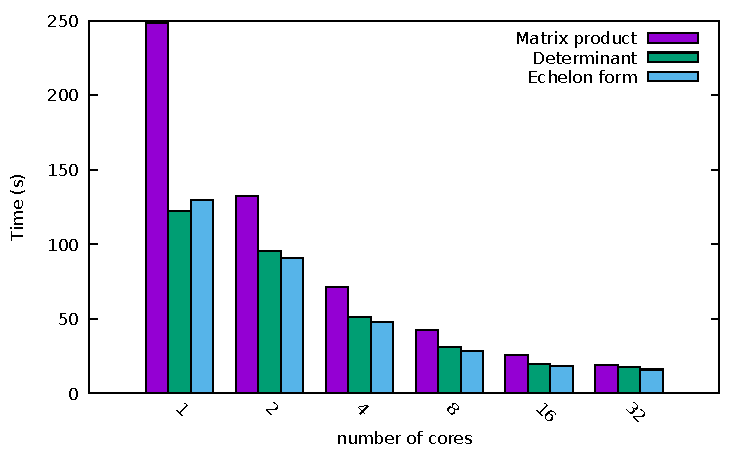
\includegraphics[width=.8\textwidth]{Pictures/histo_bigfoot3}
    \caption{Parallel computation time for some finite field linear algebra operations in SageMath on a 32 core Intel
      Xeon 6130 Gold. Matrices are $20\,000\times 20\,000$ with full rank over $\mathbb{Z}/1\,048\,573\mathbb{Z}$. }
    \label{fig:histo_sage}
  \end{center}
\end{figure}
The speed-up relative to a single threaded run of these timings is reported in Figure~\ref{fig:speedup_sage}
\begin{figure}[htb]
  \begin{center}
    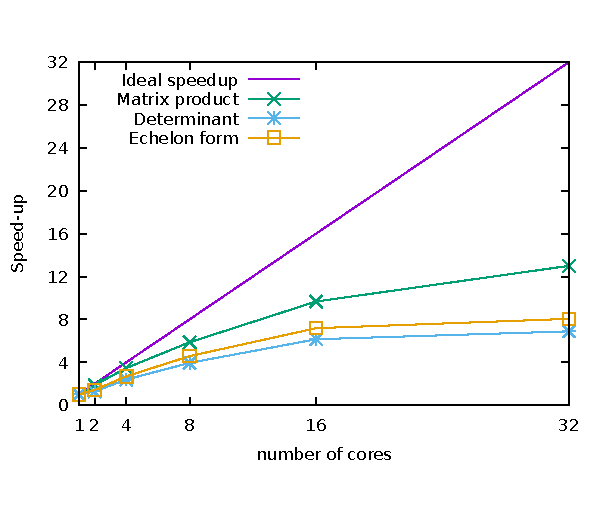
\includegraphics[width=.7\textwidth]{Pictures/speedup_bigfoot3}
    \caption{Parallel speedup for some finite field linear algebra operations in SageMath on a 32 core Intel
      Xeon 6130 Gold. Matrices are $20\,000\times 20\,000$ with full rank over $\mathbb{Z}/1\,048\,573\mathbb{Z}$.}
    \label{fig:speedup_sage}
  \end{center}
\end{figure}

The scalability shown on Figure~\ref{fig:speedup_sage} is good but not close to the best theoretical linear
speedup. This comes from the following reasons:
\begin{itemize}
\item first, the interface between the system \SageMath (running an interactive ipython) and the compiled code of the
  library has adds a constant overhead despite our efforts to reduce it as much as possible. According to Amdhal's law,
  such an overhead severely penalizes the speedup measured;
\item the use of sub-cubic arithmetic for the sequential matrix product tasks implies that the workload increases with
  the number of cores. Therefore, the true ideal speed-up curve should lie slightly below the main diagonal;
\item we did not disable the turbo-boost on this server. Consequently, runs on few cores are likely executed at a higher
  clock frequency, hence penalizing the speedup for large number of cores.
\end{itemize}

Still, these timings show that very high performances can be attained directly from the high level interface of
\SageMath, for instance the computation speed on 32 cores reaches 838Gfops for matrix multiplication and 301 Gfops for
the determinant.


\bibliographystyle{acm}
\bibliography{D3.11}
\end{document}

%%% Local Variables:
%%% mode: latex
%%% TeX-master: t
%%% End:

